\documentclass[14pt]{extbook}
\usepackage{multicol, enumerate, enumitem, hyperref, color, soul, setspace, parskip, fancyhdr} %General Packages
\usepackage{amssymb, amsthm, amsmath, latexsym, units, mathtools} %Math Packages
\everymath{\displaystyle} %All math in Display Style
% Packages with additional options
\usepackage[headsep=0.5cm,headheight=12pt, left=1 in,right= 1 in,top= 1 in,bottom= 1 in]{geometry}
\usepackage[usenames,dvipsnames]{xcolor}
\usepackage{dashrule}  % Package to use the command below to create lines between items
\newcommand{\litem}[1]{\item#1\hspace*{-1cm}\rule{\textwidth}{0.4pt}}
\pagestyle{fancy}
\lhead{Progress Quiz 8}
\chead{}
\rhead{Version A}
\lfoot{5493-4176}
\cfoot{}
\rfoot{Summer C 2021}
\begin{document}

\begin{enumerate}
\litem{
First, find the equation of the line containing the two points below. Then, write the equation in the form $ y=mx+b $ and choose the intervals that contain $m$ and $b$.\[ (3, 8) \text{ and } (4, 2) \]\begin{enumerate}[label=\Alph*.]
\item \( m \in [-11, -5] \hspace*{3mm} b \in [26, 27] \)
\item \( m \in [3, 9] \hspace*{3mm} b \in [-24, -21] \)
\item \( m \in [-11, -5] \hspace*{3mm} b \in [-10, -1] \)
\item \( m \in [-11, -5] \hspace*{3mm} b \in [-26, -23] \)
\item \( m \in [-11, -5] \hspace*{3mm} b \in [4, 8] \)

\end{enumerate} }
\litem{
Solve the equation below. Then, choose the interval that contains the solution.\[ -14(2x -19) = -10(17x -16) \]\begin{enumerate}[label=\Alph*.]
\item \( x \in [-3.01, -2.31] \)
\item \( x \in [2.85, 3.54] \)
\item \( x \in [2.03, 2.61] \)
\item \( x \in [-0.76, -0.56] \)
\item \( \text{There are no real solutions.} \)

\end{enumerate} }
\litem{
Write the equation of the line in the graph below in Standard Form $Ax+By=C$. Then, choose the intervals that contain $A, B, \text{ and } C$.
\begin{center}
    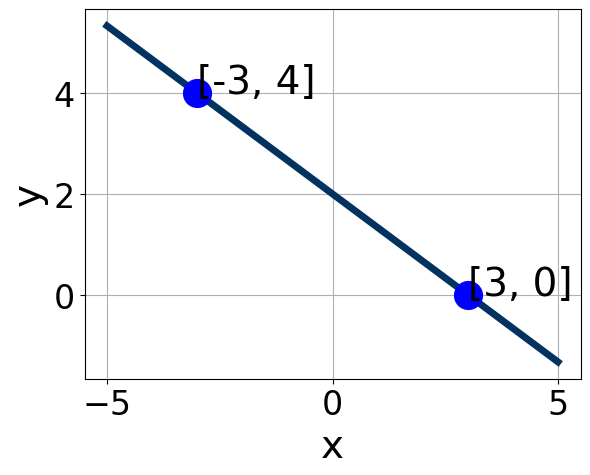
\includegraphics[width=0.5\textwidth]{../Figures/linearGraphToStandardA.png}
\end{center}
\begin{enumerate}[label=\Alph*.]
\item \( A \in [1.75, 2.91], \hspace{3mm} B \in [-3.69, -2.65], \text{ and } \hspace{3mm} C \in [-6.6, -2.8] \)
\item \( A \in [0.41, 1.52], \hspace{3mm} B \in [0.76, 1.89], \text{ and } \hspace{3mm} C \in [1, 3.1] \)
\item \( A \in [0.41, 1.52], \hspace{3mm} B \in [-1.97, -0.93], \text{ and } \hspace{3mm} C \in [-3.9, 0.2] \)
\item \( A \in [1.75, 2.91], \hspace{3mm} B \in [2.11, 4.64], \text{ and } \hspace{3mm} C \in [5.6, 7.5] \)
\item \( A \in [-2.7, -0.81], \hspace{3mm} B \in [-3.69, -2.65], \text{ and } \hspace{3mm} C \in [-6.6, -2.8] \)

\end{enumerate} }
\litem{
Find the equation of the line described below. Write the linear equation in the form $ y=mx+b $ and choose the intervals that contain $m$ and $b$.\[ \text{Parallel to } 8 x - 5 y = 12 \text{ and passing through the point } (-6, -5). \]\begin{enumerate}[label=\Alph*.]
\item \( m \in [1.37, 1.62] \hspace*{3mm} b \in [-7.6, -3.6] \)
\item \( m \in [0.41, 0.7] \hspace*{3mm} b \in [2.6, 5.6] \)
\item \( m \in [-1.74, -0.49] \hspace*{3mm} b \in [-18.6, -11.6] \)
\item \( m \in [1.37, 1.62] \hspace*{3mm} b \in [0, 2] \)
\item \( m \in [1.37, 1.62] \hspace*{3mm} b \in [2.6, 5.6] \)

\end{enumerate} }
\litem{
Solve the linear equation below. Then, choose the interval that contains the solution.\[ \frac{-7x + 4}{3} - \frac{-6x -5}{2} = \frac{5x + 7}{5} \]\begin{enumerate}[label=\Alph*.]
\item \( x \in [4.5, 6.5] \)
\item \( x \in [-9.6, -6.7] \)
\item \( x \in [-1.4, 1.5] \)
\item \( x \in [6.6, 7.6] \)
\item \( \text{There are no real solutions.} \)

\end{enumerate} }
\litem{
Find the equation of the line described below. Write the linear equation in the form $ y=mx+b $ and choose the intervals that contain $m$ and $b$.\[ \text{Parallel to } 4 x - 7 y = 14 \text{ and passing through the point } (-8, -6). \]\begin{enumerate}[label=\Alph*.]
\item \( m \in [-0.02, 0.95] \hspace*{3mm} b \in [1.67, 2.54] \)
\item \( m \in [1.64, 2.32] \hspace*{3mm} b \in [-1.62, -1.29] \)
\item \( m \in [-0.02, 0.95] \hspace*{3mm} b \in [-0.04, 1.6] \)
\item \( m \in [-0.02, 0.95] \hspace*{3mm} b \in [-1.62, -1.29] \)
\item \( m \in [-1.06, 0.39] \hspace*{3mm} b \in [-11.81, -8.98] \)

\end{enumerate} }
\litem{
Solve the equation below. Then, choose the interval that contains the solution.\[ -17(-16x -3) = -14(-7x -4) \]\begin{enumerate}[label=\Alph*.]
\item \( x \in [-0.22, 0.15] \)
\item \( x \in [-0.33, -0.2] \)
\item \( x \in [-0.79, -0.61] \)
\item \( x \in [0.34, 0.76] \)
\item \( \text{There are no real solutions.} \)

\end{enumerate} }
\litem{
First, find the equation of the line containing the two points below. Then, write the equation in the form $ y=mx+b $ and choose the intervals that contain $m$ and $b$.\[ (-9, 6) \text{ and } (-5, -4) \]\begin{enumerate}[label=\Alph*.]
\item \( m \in [1.5, 5.5] \hspace*{3mm} b \in [8.2, 9.8] \)
\item \( m \in [-6.5, -1.5] \hspace*{3mm} b \in [0.9, 1.2] \)
\item \( m \in [-6.5, -1.5] \hspace*{3mm} b \in [-18.8, -14.7] \)
\item \( m \in [-6.5, -1.5] \hspace*{3mm} b \in [16, 16.9] \)
\item \( m \in [-6.5, -1.5] \hspace*{3mm} b \in [13.6, 15.9] \)

\end{enumerate} }
\litem{
Write the equation of the line in the graph below in Standard Form $Ax+By=C$. Then, choose the intervals that contain $A, B, \text{ and } C$.
\begin{center}
    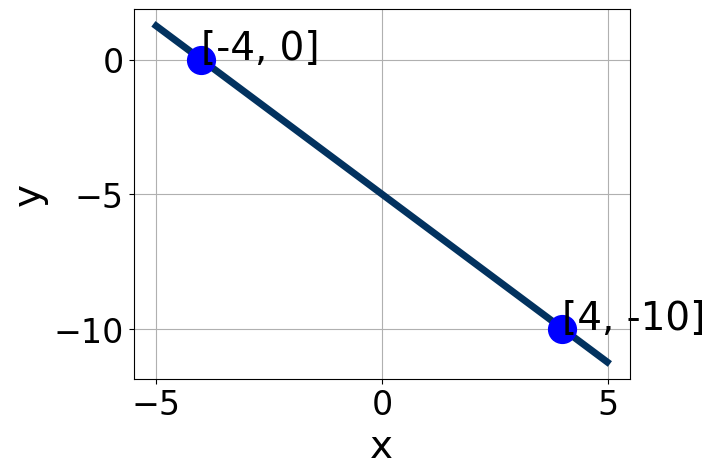
\includegraphics[width=0.5\textwidth]{../Figures/linearGraphToStandardCopyA.png}
\end{center}
\begin{enumerate}[label=\Alph*.]
\item \( A \in [-1.3, 3.1], \hspace{3mm} B \in [-0.06, 1.87], \text{ and } \hspace{3mm} C \in [-6, 1] \)
\item \( A \in [-1.3, 3.1], \hspace{3mm} B \in [-1.57, -0.25], \text{ and } \hspace{3mm} C \in [4, 6] \)
\item \( A \in [3.1, 8.7], \hspace{3mm} B \in [3.44, 4.03], \text{ and } \hspace{3mm} C \in [-21, -19] \)
\item \( A \in [-5.6, -4.8], \hspace{3mm} B \in [-4.51, -2.73], \text{ and } \hspace{3mm} C \in [12, 24] \)
\item \( A \in [3.1, 8.7], \hspace{3mm} B \in [-4.51, -2.73], \text{ and } \hspace{3mm} C \in [12, 24] \)

\end{enumerate} }
\litem{
Solve the linear equation below. Then, choose the interval that contains the solution.\[ \frac{4x + 6}{3} - \frac{4x + 6}{7} = \frac{3x + 4}{8} \]\begin{enumerate}[label=\Alph*.]
\item \( x \in [-2.8, -1.6] \)
\item \( x \in [9.8, 10.6] \)
\item \( x \in [-6.2, -5.6] \)
\item \( x \in [-0.1, 2] \)
\item \( \text{There are no real solutions.} \)

\end{enumerate} }
\end{enumerate}

\end{document}